\documentclass[a4paper,11pt,oneside]{report}
\usepackage{geometry}
\usepackage[english]{babel}
\usepackage[utf8]{inputenc}
\usepackage{hyperref}
\usepackage{amsmath}
\usepackage{amssymb}
\usepackage[T1]{fontenc}
\usepackage{relsize}
\usepackage{lettrine}
\usepackage{fullpage}
\usepackage{multicol}
\usepackage{hyperref}
\usepackage{graphicx}
\usepackage{color}
\usepackage[T1]{fontenc}
\usepackage{relsize}
\usepackage{kpfonts}
\usepackage{caption}
\usepackage[footnote,smaller]{acronym}
\usepackage[perpage]{footmisc}
\usepackage[]{titlesec}
\usepackage[xindy,toc]{glossaries}
\usepackage{natbib}
\usepackage{fancyvrb}
\usepackage{float}
\definecolor{gris25}{gray}{0.75}
\hypersetup{colorlinks=true, urlcolor= blue, linkcolor= blue}


% % % Pour avoir plus de figures
\renewcommand\floatpagefraction{.9}
\renewcommand\topfraction{.9}
\renewcommand\bottomfraction{.9}
\renewcommand\textfraction{.1}   
\setcounter{totalnumber}{50}
\setcounter{topnumber}{50}
\setcounter{bottomnumber}{50}


% % % Géométrie de la page
\setlength\leftmargini{1.5em} % premier niveau
\setlength\leftmarginii{2.2em} % 2ème niveau

% Changements de commandes utiles
\renewcommand*{\acsfont}[1]{\brand{#1}}
\newcommand{\brand}[1]{\textsc{\textbf{#1}}}

\let\oldpar\paragraph
\renewcommand{\paragraph}[1]{\oldpar{#1}\mbox{}\\}

\title{
\begin{figure} [h!]
\begin{center}

\includegraphics[width=0.4\textwidth]{LogoUniversiteBX1.jpg}
\end{center}	
\end{figure}
\textbf{\large{Université of Bordeaux \\
		 2013-2014}			 	  		
\paragraph{}
\LARGE{Projet d'Étude et de Recherche}
\paragraph{}
\Huge{\textcolor{red}{Three-dimensional musical instrument}}}
\newline
\newline
 \large{\textbf{\textit{Supervisor:}} Aurélie \textsc{Bugeau}}\\
 \large{\textbf{\textit{Clients:}} Myriam \textsc{Desainte-Catherine}, Joseph
 \textsc{Larralde}, and Florent \textsc{Berthaut}}}


\author{\fcolorbox{gris25} {gris25} {\small{Mohamed \textsc{Bourara}, Jean \textsc{Bui-Quang}, Omar \textsc{Ourhi}, Jean-Michaël \textsc{Celerier}, Marie \textsc{Immacula Omiscar} and Damien \textsc{Clergeaud}}}}

\date{\fcolorbox{gris25} {gris25} {\today}}

\acrodef{LaBRI}{Laboratoire Bordelais de Recherche en Informatique}
\acrodef{SCRIME}{Studio de Création et de Recherche en Informatique et Musique Électroacoustique}
\acrodef{HMD}{Head-mounted Display}
\acrodef{CAVE}{CAVE Automatic Virtual Environment}

\makeglossaries
\begin{document}
\maketitle
\vspace{5cm}

\tableofcontents
\listoffigures
\newglossaryentry{display}
{
  name=display,
  description={something that can convert data as a byte stream into light, in order to be perceived by an human eye}
}
\section{Introduction}
\begin{frame}
  \begin{itemize}
  \item \textbf{Context} : Conceiving a modern musical instrument that can be used in conjunction with a 3D display.

  \item{\textbf{Goals} :
    \begin{itemize}
    \item Understand 3D displays technologies
    \item Implement 3D-enabled visualization methods for two new musical instruments : DRILE and the Aerial Percussion
    \end{itemize}
  }

  \item{\textbf{Problem} : There are numerous kind of 3D displays. What is the most adapted to the situation ?}
  \end{itemize}
\end{frame}


\chapter{Subject and definitions}
\section{Subject presentation}
\paragraph{3D Musical instruments}
At the \ac{SCRIME} and \ac{LABRI}, three-dimensional musical instruments have been implemented within the context of research in interactive virtual reality and music computing. 

The \brand{Drile} \cite{berthaut2010drile} is a 3D musical instrument which allows manipulation of the structure of a song using \gls{livelooping}, in an immersive virtual reality scene.

The \brand{Aerial Percussion} is a 3D musical instrument which generates sounds using the position in space of sensors which are put at the end of drumsticks. Virtual 3D shapes like cubes, cylinders, are positionned around the instrument and the musician. According to the position, the orientation, and the speed of the sensors, sounds are generated.

\paragraph{Objectives}
We were asked to implement a prototype of a 3D render and display device, for musical performance.
It is necessary to take into account the constraints inherent to a musical performance environment, as well as the constraints of the instruments.

Here are some constraints for the performance : 
\begin{itemize}
\item The musician has to be in front of the audience.
\item The musician requires visual cues inherent to the utilisation of the instrument, and the audience must see the instrument to understand the gestures and actions of the musician.
\end{itemize}

To enact this implementation, a precise explanation of the nature of the 3D musical instruments is required.

\paragraph{Plan for this section}
We will first make a short presentation of 3D musical instruments, present and will then define the concepts of immersivity and interactivity.

\newpage
\section{What is a 3D musical instrument?}
{\LARGE{TODO a reformuler : bof le wikipédia}}\\
A 3D musical instrument, or an immersive virtual musical instrument, represents sound processes and their parameters as 3D entities of a virtual reality so that they can be perceived not only through auditory feedback but also visually in 3D and possibly through touch as well as haptic feedback, using 3D interface metaphors consisting of interaction techniques such as navigation, selection and manipulation.

\paragraph{Example for the Drile}
For instance, the picture \ref{fig:drile} shows a musician with special glasses, as well as joysticks with force-feedback haptic sensors (Piivert \cite{berthaut2010piivert}). 
The user handles 3D shapes in a 3D environement to influence the music generation. A specific part of this report will be dedicated to a precise study of the \brand{Drile}.

\begin{figure}[t]
\centering
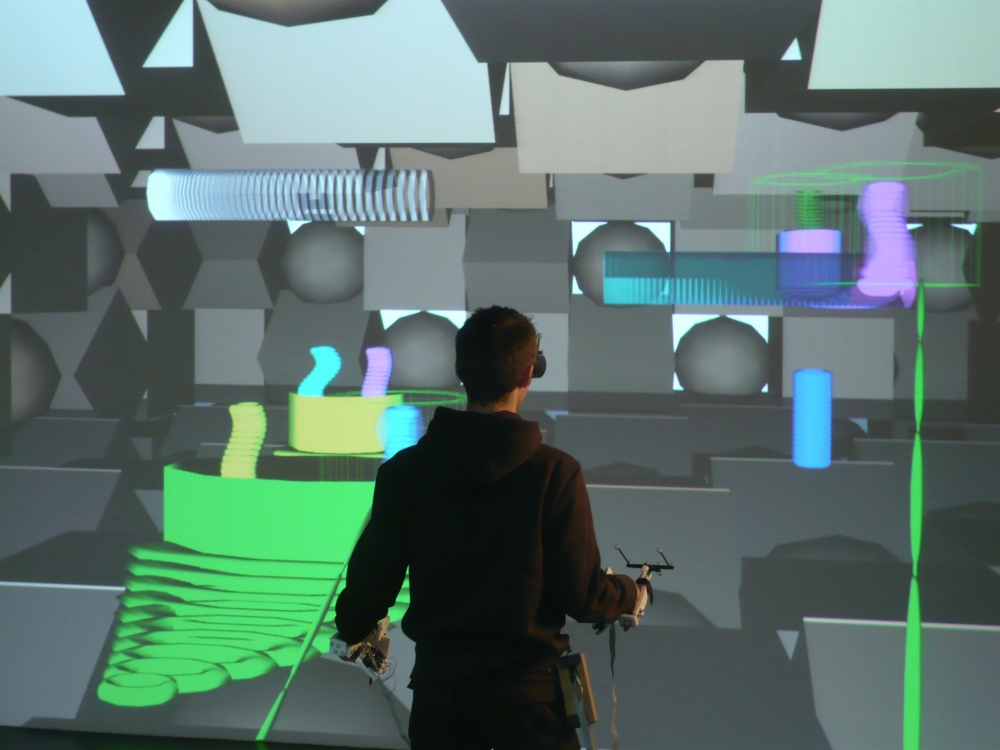
\includegraphics[scale=0.3]{image/drile.jpg}
\caption{Picture of a musician using DRILE}
\label{fig:drile}
\end{figure}

\newpage
\section{Immersion}
\paragraph{Definition}
Immersion is a psychologic state where the subject stops about taking care of its own physical state.
The immersion is quite important in virtual reality. For instance, for the Aerial Percussion, it would come down to the state the performer is when he stops thinking consciously of the disposition of the shapes he interacts with. The musician will then be immersed in the virtual 3D environment which consists in the shapes disposition.

Hence, to immerse an user, multiple parameters are accessible to the 3D instrument designer. 
They are mostly linked to the senses of the human body. In our project, we will mainly focus on vision, and more precisely on 3D display devices.

\paragraph{Interactivity \& reactivity}
Interactivity is an important aspect of the immersion capacities of a musical system.
The user is more likely to get an immersive feeling in a virtual world, if the world instantly reacts to his actions and gestures \cite{biocca1995immersive}.
This leads us to an important part of the 3D musical instrument : the interface, the controls that the performer requires to operate the instrument.

\section{Control}
In order to understand and define what is the control of a 3D musical instrument, it is necessary to think of the instrument in two different ways : 
\begin{enumerate}
\item First of all, it is a musical instrument, which implies multiples constraints :
\begin{itemize}
\item It has to be adapted to the human body shape so that the musican can manipulate it.
\item It has to be precise enough for the performer to be able to learn how to play the instrument.
\end{itemize}
\item But it is also an interactive immersive system, which means that it requires :
\begin{itemize}
\item A lot of interactivity.
\item The usage of senses for a feedback : for instance, immersive visual and haptic feedback (as well as auditive, since it is a musical instrument).
\end{itemize} 
\end{enumerate}

\paragraph{Musical instrument gestures}
In order to conceive a 3D musical instrument, it is necessary to understand the movements that the musician does while playing. For instance, the Cadoz gesture segmentation \cite{cadoz1999musique} is an attempt to differentiate different families of gestures while playing.

Cadoz defines three kinds of gestures that all come to play when playing music:

\begin{itemize}
\item Selection gestures : The musician selects a component of the instrument that he will play on. For instance, for stringed musical instruments, where the same tone can be achieved on different strings, but with a different timber, it is the choice of the string on which the note will be played.
\item Modification gestures : It is an action that modifies the physical state of the instrument. For instance, it would be the case of the guitar player who presses its hand on the guitar strings against the wood. 
\item Excitation gestures : These actions are the ones generating the actual sound of the instrument, by making the air vibe. On a guitar, it would be picking a string, and on a violin, it would be moving the bow against a string. This gesture is the one the artist can put expression inside : for instance, a violonist can press his bow softly or hardly, in order to change the nuance.
\end{itemize}

\paragraph{Control and immersion}
In order to correctly play an instrument, the user requires some kind of manipulation comfort : it must not be painful or too tiring to play. 
Hence the requirement for immersion : being immersed means that the user does not need to put effort into playing the 3D musical instrument, he becomes part of it.
An easy way to improve immersion is to make the environment react to the performer's movements. 

This can be achieved by using head tracking, with a \brand{Kinect} for instance, or a \ac{HMD}, a \ac{CAVE} or other virtual reality devices and methods like Fishtank VR \cite{robertson1997immersion}. This allows to adapt the scene's projection to the movements of the head of the user : for instance, if he turns his head to the right, the display will adapt by showing him what he would see if it was real.

Haptic feedback buttons also increase the consciousness of the user's actions, which implies an increased precision.

Florent Berthaut thought about most of these problematics while conceiving \brand{Piivert} \cite{berthaut2010piivert}, the control interface to the \brand{Drile}.
 % Relation avec instrus 3D
\chapter{Three-dimensional displays}
\label{chap:3ddisp}
\section{Definition of a 3D display}
While it is commonplace to hear about 3D display in television or smartphone advertisement nowadays, the distinction between 2D and 3D might be more difficult to settle.
\subsection{The problem}
If we take the simple definition : a 3D display is a display that can show 3D images, it is really ambiguous, because of what is supposed to be "3D". For instance, for years, video games have been advertising 3D engines and spectacular 3D graphics, even without the depth provided by what is now called 3D displays or 3D movies in cinema.
Another litteral but limited definition for a 3D display would be a display that really exists in three-dimensions; one could think for instance of programmable matter and claytronics, or at least of a display that would be able to show a scene or an object from any point of view.

Hence, we have to qualify what is 3D and what it is not, in order to build a real definition.

\subsection{Parameters}
In the litterature, the main idea is to relate to the human brain and body capabilities to define 3D vision (\cite{okoshi1976three}, \cite{pimenta2012comprehensive}). For instance, a big part of the "3D" feel is due to the fact of having two eyes that looks in the same direction, but from a slightly different angle, but it is not the only parameter.

The visual cues of 3D vision are separated in two families:  
\begin{itemize}
\item Physiological cues. They will relate to the capabilities of the human body.
\item Psychological cues. They will relate to the information inference capabilities of the human brain.
\end{itemize}
\subsection{Presentation of common visual cues}
Most of the visual cues on \ref{fig:visualcues} are explained in-depth in \cite{pimenta2012comprehensive}, however a short explanation is provided in the glossary for many of them.
\begin{figure}[h!]
\centering
\begin{tabular}{lr}
\begin{tabular}{|c|}
\hline
Psychological cues \\
\hline
\Gls{occlusion} \\
\Gls{linpersp} \\
\Gls{atmpersp} \\
\Gls{shading} \\
\Gls{motionparallax} \\
\Gls{kineticdepth} \\
\hline
\end{tabular} & 
\begin{tabular}{|c|}
\hline
Physiological cues \\
\hline
\Gls{stereoscopy} \\
\Gls{convergence} \\
\Gls{accomodation} \\
Retinal image size \cite{mehrabi2013making} \\
Texture gradient \cite{howard2012perceiving} \\
\hline
\end{tabular}
\end{tabular}
\caption{Common visual cues}
\label{fig:visualcues}
\end{figure}

A complete classification of the current state of the art in 3D displays using these visual cues is present in \cite{mehrabi2013making} on Table 2.

\subsection{Definition of a 3D display}
The definition retained in \cite{pimenta2012comprehensive} is the following : a 3D display is a display that uses at least one of the physiological cues. We will see that most of the displays use the stereoscopy cue, because it is the one that provides the most convincing 3D experience\cite{kaufman122006perceptual}.

\section{Classification of the 3D displays}
One of the main problem while trying to find a proper \gls{display} for a given application is to choose a relevant classification for the displays, that allows a choice with criterions relevant to the application.
\subsection{Criterions}
There was a lack of proper nomenclature in the literature for a long time \cite{pimenta2012comprehensive}. However, some attemps have been made to find relevant criterions that would be general enough to cover the current display techniques, but also the ones that are not yet thought of.

\subsubsection{Different classifications}
The first classification was in \cite{okoshi1976three}, and it was really based upon the different kinds of displays existing at the time: 
\begin{itemize}
\item Lens-sheet three dimensional pictures.
\item Projection-type three dimensional displays.
\item Holography.
\end{itemize}

However, it did not hold well against the emergence of new techniques, like volumetric displays for instance.

Other classifications %\cite{ref nécessaire} 
would limit themselves to only a subset of 3D displays.

Hence the need for a classification that would not base itself on the different technologies, but on criterions that would be inherent to the idea of display and human vision.

\subsubsection{Chosen classification}
In \cite{pimenta2012comprehensive}, the main idea is to classify the displays according to two axes : 

\begin{itemize}
\item The display depth (flat or deep).
\item The number of points of view from which the image can be seen (duoscopic, multiscopic, or omniscopic).
\end{itemize}

\section{In-depth presentation of some 3D display methods}
This section describes the different technologies used by manufacturers of 3D displays, and also explains some 3D visualization systems in detail. But first we will define what are stereoscopic and auto-stereoscopic displays. \\
\textbf{Stereoscopy} is the set of techniques used to reproduce a depth perception from two planar images.\\
\textbf{Autostereoscopy} is a method of image representation, either in three-dimension or stereoscopic, which requires no additional device to render the 3D effect. 

\subsection{Two-view 3D displays}
Since a decade, a new generation of screens appeared: 3D screens. The main feature of these screens, which distinguishes them from conventional screens, is their ability to display stereoscopic images : each eye of the observer will receive a different point of view.
There are multiple technologies that are able to power such screens; we will explain some. But an exhaustive list is present in \cite{mehrabi2013making}.

\subsubsection{Wavelength selective displays}
To view in 3D, it is necessary to provide our brain two images of the same scene taken from two different points of view. This is the principle of stereoscopy. The distance between the two points of view is used to compute the depth of field to achieve the 3D effect.\\
Different methods exist so that each eye receives the intended image. 

The most famous are the anaglyphic glasses, pictured on figure \ref{fig:anaglass}. However, the result is of poor quality and unpleasant after some time.

\begin{figure}[h!]
\centering
\centering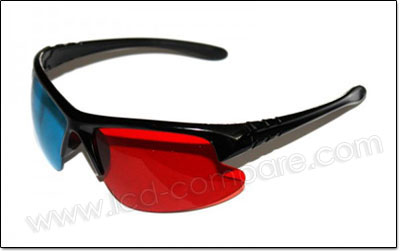
\includegraphics[width=6cm,height=40mm]{image/1.jpg}
\caption{Red/cyan color filter 3D glasses\cite{ViewingOn3D}}
\label{fig:anaglass}
\end{figure}

In this case, images are filtered by color. The two images are superimposed and the glasses incorporate a color filter. Each eye can only see the image intended for it, so this can be used to create a stereoscopic effect. 

This is a passive method.

\subsubsection{Time-sequential two-view displays}
The idea is that the images are shown one after the other, but it has two requirements : 
\begin{itemize}
\item The switching between images must be fast : a refresh rate of 48 Hz is theoretically minimal for a 24 fps movie, however research \cite{holliman2011three} shown that 58 Hz is a practical minimum.
\item Each eye must see only the images directed to it. There are multiple technologies to achieve this, passive and active.
\end{itemize}

\paragraph{Passive method}
This technique uses polarized glasses. The right lens is polarized in one direction while the left lens is polarized in the other direction. 

\begin{figure}[h!]
\begin{center}
\begin{minipage}{1\linewidth}
\centering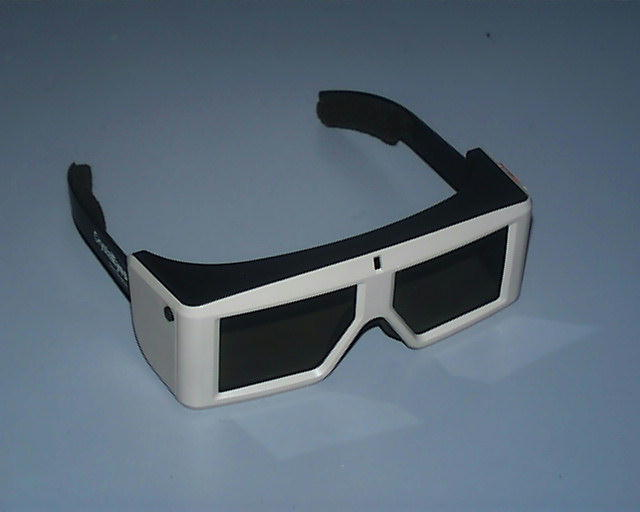
\includegraphics[width=6cm,height=30mm]{image/2.jpg}
\caption{Polarized 3D system\cite{Polarized3D}}
\end{minipage}
\end{center}
\end{figure}

This is not an expensive method, however the image is often less bright. It is generally used in movie theaters.

\paragraph{Active method}
This technique uses active glasses, with LCD shutters that needs to be synchronized with the screen refresh rate : one of the glass goes black while the other allow the light to pass, which allows the eyes to receive only the wanted image at the wanted time.

This method is more expensive, but reviews often said it offers a better experience.

\subsubsection{Time-parallel two-view displays}
This is the opposite of time-sequential two-view displays. Both eyes receive a stream of images at the same time.

\paragraph{Simple stereoscopy}
There are multiple designs available. One would be a variation on the polarized glasses : instead of having the images one after the other, they are put together, for instance by using a dual projector. However, this can lead to crosstalk.

Another design uses multiple LCD displays, one seen in transmission and the other in reflection in a mirror, in order to change the polarization of the reflected screen.

\paragraph{Auto-stereoscopy}
This technique is interesting, because no special headgear is required : the correct light information is sent directly by the screen to the eyes.

However, the viewer has to be at a precise position in front of the screen for it to work. Hence, it only works with a single person except in the case of a very large and expensive screen.

Some recent designs can for instance use reflective screens \cite{smithwick2013autostereoscopic}.

\subsection{Horizontal parallax multiview 3D diplays}
Multiview or multiscopic displays are displays that can be seen from a finite number of point of view and show a different picture corresponding to this point of view.

There are two main types of technology for multiview parallax displays: either by applying a parallax barrier, or by application of a lenticular panel.

A parallax barrier is a mask of parallel black stripes that reveals the different parts of the underlying image depending on the direction of observation.

The same effect can be obtained with the lenticular sheets, which are linear networks of narrow cylindrical lenses. Both techniques are used to show a unique view of each position in the viewing area. Thus, a viewer feels the motion parallax and binocular stereo without the use of special glasses. 

\subsubsection{Lenticular Displays}
The application of a lenticular panel to deflect the rays from the pixels of the screen in order to reproduce a stereoscopic display giving the images an impression of depth.

A lenticular panel is composed of a regular grid of small spherical lenses. Each lens covers an area of several pixels of the flat screen and will divert the direction of the light emitted by the pixels covered.

As we can see on figure \ref{fig:lenticular}, each eye only sees the right or left pixels. An observer looking at a lenticular 3D screen does not see the same screen pixel between his left eye and his right eye, although both eyes see the same lenses.

With horizontal lenses, projecting changing images, the perceived image depends on the angle between the eye and the lenses.

\begin{figure}[h!]
\centering
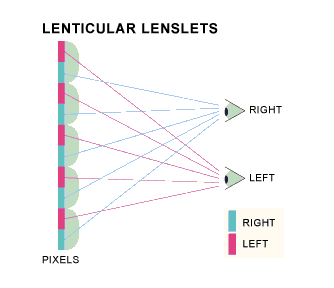
\includegraphics[width=8cm,height=5cm]{image/lentuc.png}
\caption{A lens array\cite{glasses-free3D}}

\label{fig:lenticular}
\end{figure}

\subsubsection{Parallax Barrier Displays}
Instead of lenses, multiple small masks are put in front of the pixels. The images are divided into columns of a width of one pixel.
Each mask is precisely placed so that the observer, himself set at the correct distance from the screen, views the image that corresponds to each eye. 

Thanks to the cache, an image is sent to the right eye and another in the left eye, as in figure \ref{fig:paraba}; the brain recreates the 3D picture by stereopsis.

In comparison with the lens array, we can see each spherical lens replaced by an opaque surface and a small hole in its center. Therefore, as in the case of the lens array, an observer looking at a small hole in the 3D screen does not see the same screen pixel between his left eye and his right eye: this is because the parallax barrier is not contiguous to the flat screen, but there is a distance of a few millimeters between the two panels.
\clearpage

\begin{figure}[h!]
\centering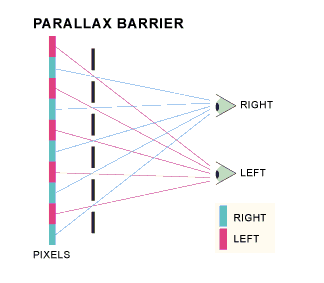
\includegraphics[width=8cm,height=5cm]{image/parallax.png}
\caption{A parallax barrier\cite{glasses-free3D}}
\label{fig:paraba}
\end{figure}

This technique provides a 3D vision without wearing glasses.

However, there are some disadvantages :
\begin{itemize}
\item It must be placed precisely over the screen, if the observer is not in a precise position, he will see superimposed images which will make thie miage look garbled.
\item Hence, movement is not compatible with this system, but it is very difficult for human beings to stay still for the length of a movie, for instance.
\item It does not allow visualization of stereoscopic image for multiple viewers at the same time.
\item Brightness is generally lower due to most of the light being occluded by the maks. However, a recent amelioration on this technique greatly improves brightness\cite{lv2014shared}.
\end{itemize}

\subsubsection{Multi-Projector Displays}
This method consists in positioning several projectors in a circle. They all display the image under a different angle. The images are projected onto a special screen. For instance, a double lenticular lens example (a spherical lens) works well, but the easiest way is to project these images on a cylindrical fog, as in figure \ref{fig:cilfog}.

\begin{figure}[h!]
\centering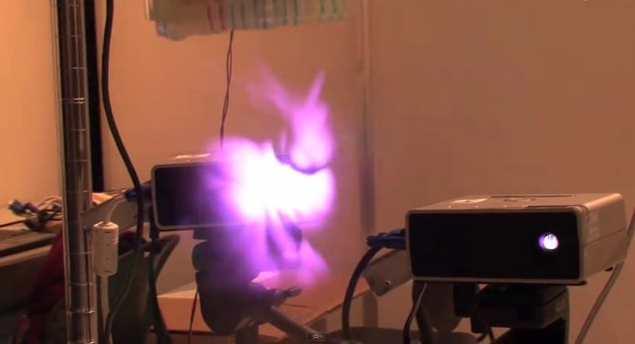
\includegraphics[width=6cm,height=4cm]{image/lapin.png}
\caption{3D multiviewpoint display\cite{3Dmultiviewpoint}}
\label{fig:cilfog}
\end{figure}

In this example, is possible to turn around the rabbit in 3 dimensions and view it from every angle.

This technique has some advantages : 
\begin{itemize}
\item There is no limit of size for the projection, which makes it good for live performance.
\end{itemize}

However, it has important requirements : 
\begin{itemize}
\item Multiple projectors are needed.
\item Headlights must be precisely aligned.
\end{itemize}


%%%%%%%%%%%%%%%%%%%%%%%%%%%%%%%%%%%%%%%%%
\subsubsection{Pepper's Ghost:}
Pepper's ghost est une technique d'illusion d'optique utilisée dans le théâtre et dans certains tours de magie.\\
L'invention de cette illusion par un certain Henry Dircks remonte à 1862, il a crée un effet d'optique qui semblait faire apparaître et disparaître des fantômes sur scène.\\
La même année, John Henry Pepper, s'implique à son tour dans l'illusion après avoir vu le show de Henry Dircks. Pepper s'était rendu compte, qu'avec quelques modifications techniques, l'illusion pourrait être plus rentable pour les propriétaires de salles.\\
Le nom de cette méthode est tiré du nom de John Henry Pepper, qui a popularisé cet effet.\\
Par exemple dans le théâtre, cet illusion se produit en utilisant des plaques de verre et des effets d’éclairage. L'acteur qui incarne le fantôme ou l’apparition est placé dans une pièce sombre invisible du public (scène cachée ).
Le public peut alors voir le reflet de l'acteur. En raison de l'angle de la vitre, la réflexion semble apparaître en trois dimensions. 

\begin{figure}[h!]
\centering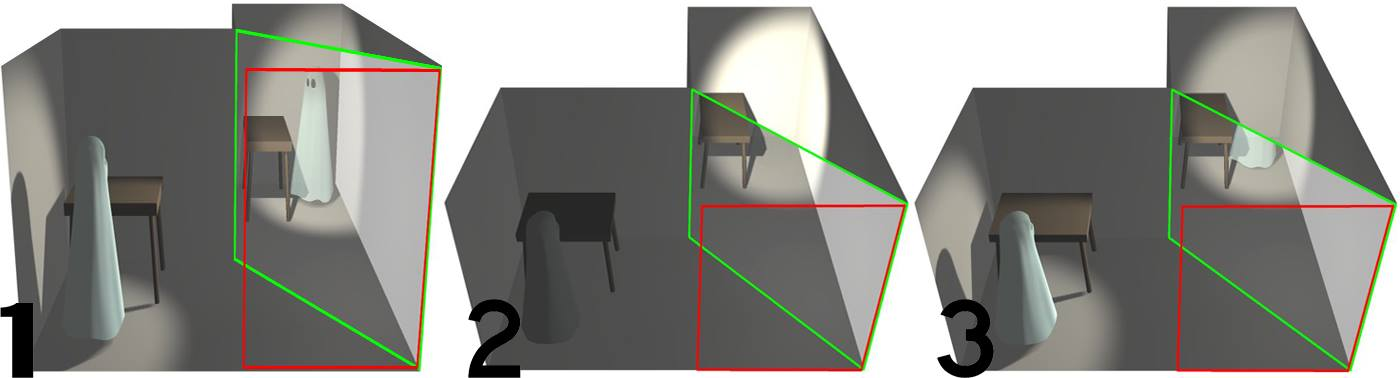
\includegraphics[width=14cm,height=4cm]{image/peppersG.jpg}
\caption{Pepper's ghost \cite{Peppers-ghost}}
\label{fig:paraba}
\end{figure}
\texbf{1-} A viewer looking through the red rectangle sees a ghost floating next to the table. The illusion is created by a large piece of glass situated at an angle between viewer and scene (green outline). The glass reflects a room hidden from the viewer (left), sometimes called a "Blue Room," that is built as mirror-image of the scene.\cite{Peppers-ghost}



%\begin{figure}[h!]
%\centering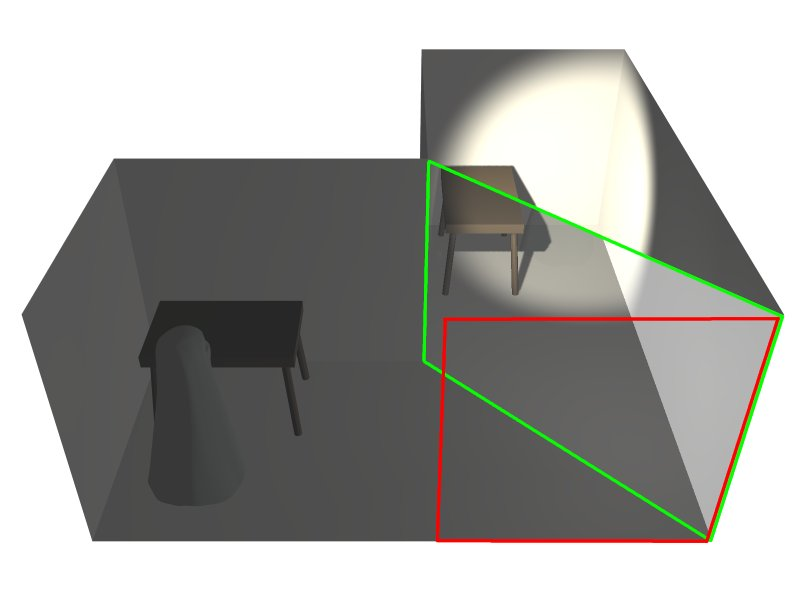
\includegraphics[width=8cm,height=5cm]{image/Peppers2.jpg}
%\caption{Pepper's ghost darkened\cite{Peppers-ghost}}
%\label{fig:paraba}
%\end{figure}
\texbf{2-} If the mirror-image room (left) is darkened, it does not reflect well in the glass. The empty room (top) is brightly lit, making it very visible to the viewer.\cite{Peppers-ghost}

%\begin{figure}[h!]
%\centering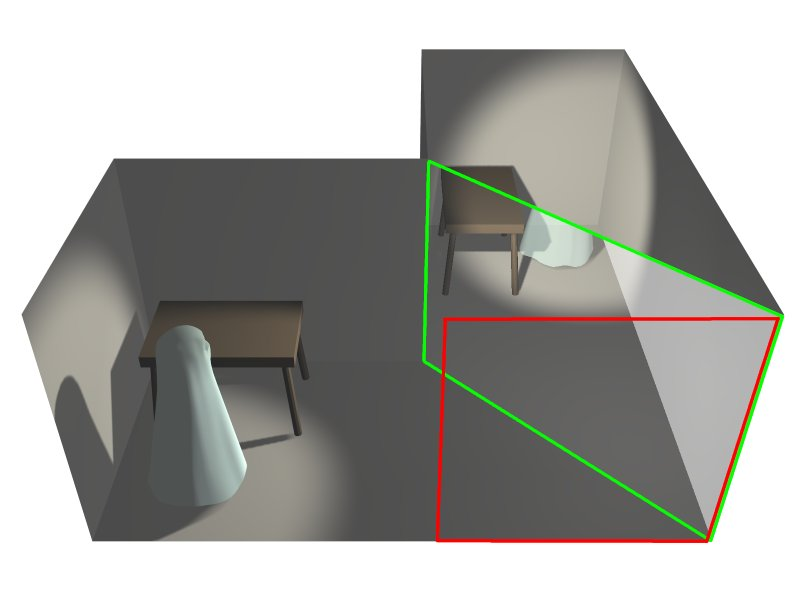
\includegraphics[width=8cm,height=5cm]{image/Peppers3.jpg}
%\caption{Pepper's ghost lit\cite{Peppers-ghost}}
%\label{fig:paraba}
%\end{figure}

\texbf{3-} When the lights in the mirror-image room are raised (with the empty room being dimmed slightly to compensate), the ghost appears out of nowhere.\cite{Peppers-ghost}\\

Aujourd’hui, la scène cachée est remplacée par un vidéo-projecteur, ce qui permet de faire apparaître des personnages ou encore des créatures imaginaires. Souvent, lorsqu’il est question d’hologrammes au théâtre, c’est du Pepper’s Ghost dont il s’agit. Il semblerait que le numérique donne une nouvelle vie au Pepper’s ghost.


\subsubsection{Glasses}
\subsubsection{Head-mounted displays}
\subsubsection{Hologram}
\subsubsection{Autostereoscopic screen}
% En rajouter à volonté % Explication des classifications
\chapter{Presentation of 3D musical instruments}
\section{History of the 3D musical instruments}
\paragraph{}
De nombreux instruments de musiques immersifs se concentrent sur la navigation dans un environnements 3D virtuelle.
Tout d'abord le projet Phase \cite{rodet2005study} explore la génération, la prise en main et le controle de son ou de musique à l'aide d'un capteur haptique et d'une représentation visuelle pouvant guidée l'utilisateur.
Un second projet, Plumage \cite{plumage2007}, est une interface pour le contrôle interactif de la composition audio spatialisées. Des plumes dispersées dans une scène 3D représente des grains sonores, générent du son lorsque des têtes de lectures les parcours. Les têtes de lectures sont contrôlées directement par l'utilisateur.
Néanmoins ces deux projets ne permettent pas de manipuler directement la structure de la synthèse sonore, mais seulement de la manipuler.
\paragraph{}
Une autre gamme d'instrument 3D se concentre sur une unique synthèse sonore. Dans ce cas nous pouvons trouver par exemple le \textit{Virtual Xylophone}, le \textit{Virutal Membrane} ou encore la \textit{Virtual Air Guitar} \cite{maki2005}. Un autre exemple d'interaction 3D avec une synthèse sonore unique est celle de Mike Wozniewski \cite{wozniewski2006spatial}. Son application permet a un utilisateur de naviguer dans une scène 3D comportant à certain point précis des générations de son. L'utilisateur entend les sons en fonction de sa position et de son orientation dans la scène 3D.
\\
La percussion aérienne est un intstrument 3D que nous pourrions mettre dans cette classe d'instrument.
\paragraph{}
Le DRILE propose une nouvelle utilisation de la 3D. Le DRILE utilise l'interaction 3D pour pouvoir manipuler plus aisément la structure même d'une musique.
\\
Le DRILE et la percussion aérienne ont été conçu pour la performance musicale.

\section{Le DRILE}
\begin{frame}
<<<<<<< HEAD
  DRILE DRILE DRILE
=======
Drile: an immersive environment for hierarchical live-looping
>>>>>>> bd6d684da1da846a2e82a6a7dce89197d6ef937c
\end{frame}

\section{Aerial Percussion}

\paragraph{}
La percussion aérienne est un instrument de musique innovant par rapport au percussion aérienne car elle ne comporte pas les fûts qu'il faut percuter pour générer le son. La position des baguettes dans l'espace est mesurée à chaque instant grâce à des capteurs. Les données obtenues sont traitées par un logiciel qui permet de détecter les impacts en temps réel et de leur associer des sons. L'utilisation d'un ordinateur permet d'obtenir une palette sonore sans limite. Elle permet aussi au musicien de s'abstraire des contraintes physique de l'instrument, il peut chorégraphier ses mouvements, la mise en scène gagne de l'importance.
Mais comment fonctionne techniquement cette instrument?

\subsection{Polhemus Liberty}

\paragraph{}
Le Polhemus Liberty est un dispositif qui permet de connaître la position et l'orientation de capteurs dans l'espace en temps réel. Un émetteur permet de générer un champ magnétique à l'aide de trois antennes fixes placées orthogonalement les unes par rapport aux autres dans un cube d'une dizaine de centimètres de côté. Ce cube, constituant la base émettrice, est relié au bloc central par un câble et est placé idéalement au centre de la zone dans laquelle les acquisitions sont faites. Le champ magnétique diffusé est capté par un second ensemble d'antennes que constitues chacun des capteurs. Ceux-ci se présentent sous la forme de petits cubes de moins d'un centimètre de côté placés au bout des câbles qui les relient au bloc central. Le signal reçu par les capteurs est ensuite échantillonné, traité pas des processeurs DSP (Digital Signal Processor) dans le bloc central, puis envoyé à l'ordinateur via celui-ci par port USB 2.0.

Tous les composants de la percussion sont sur la figure \ref{fig:percu}, de gauche à droite il y a les baguettes, le bloc central et la base émettrice.

\begin{figure}[h!]
\centering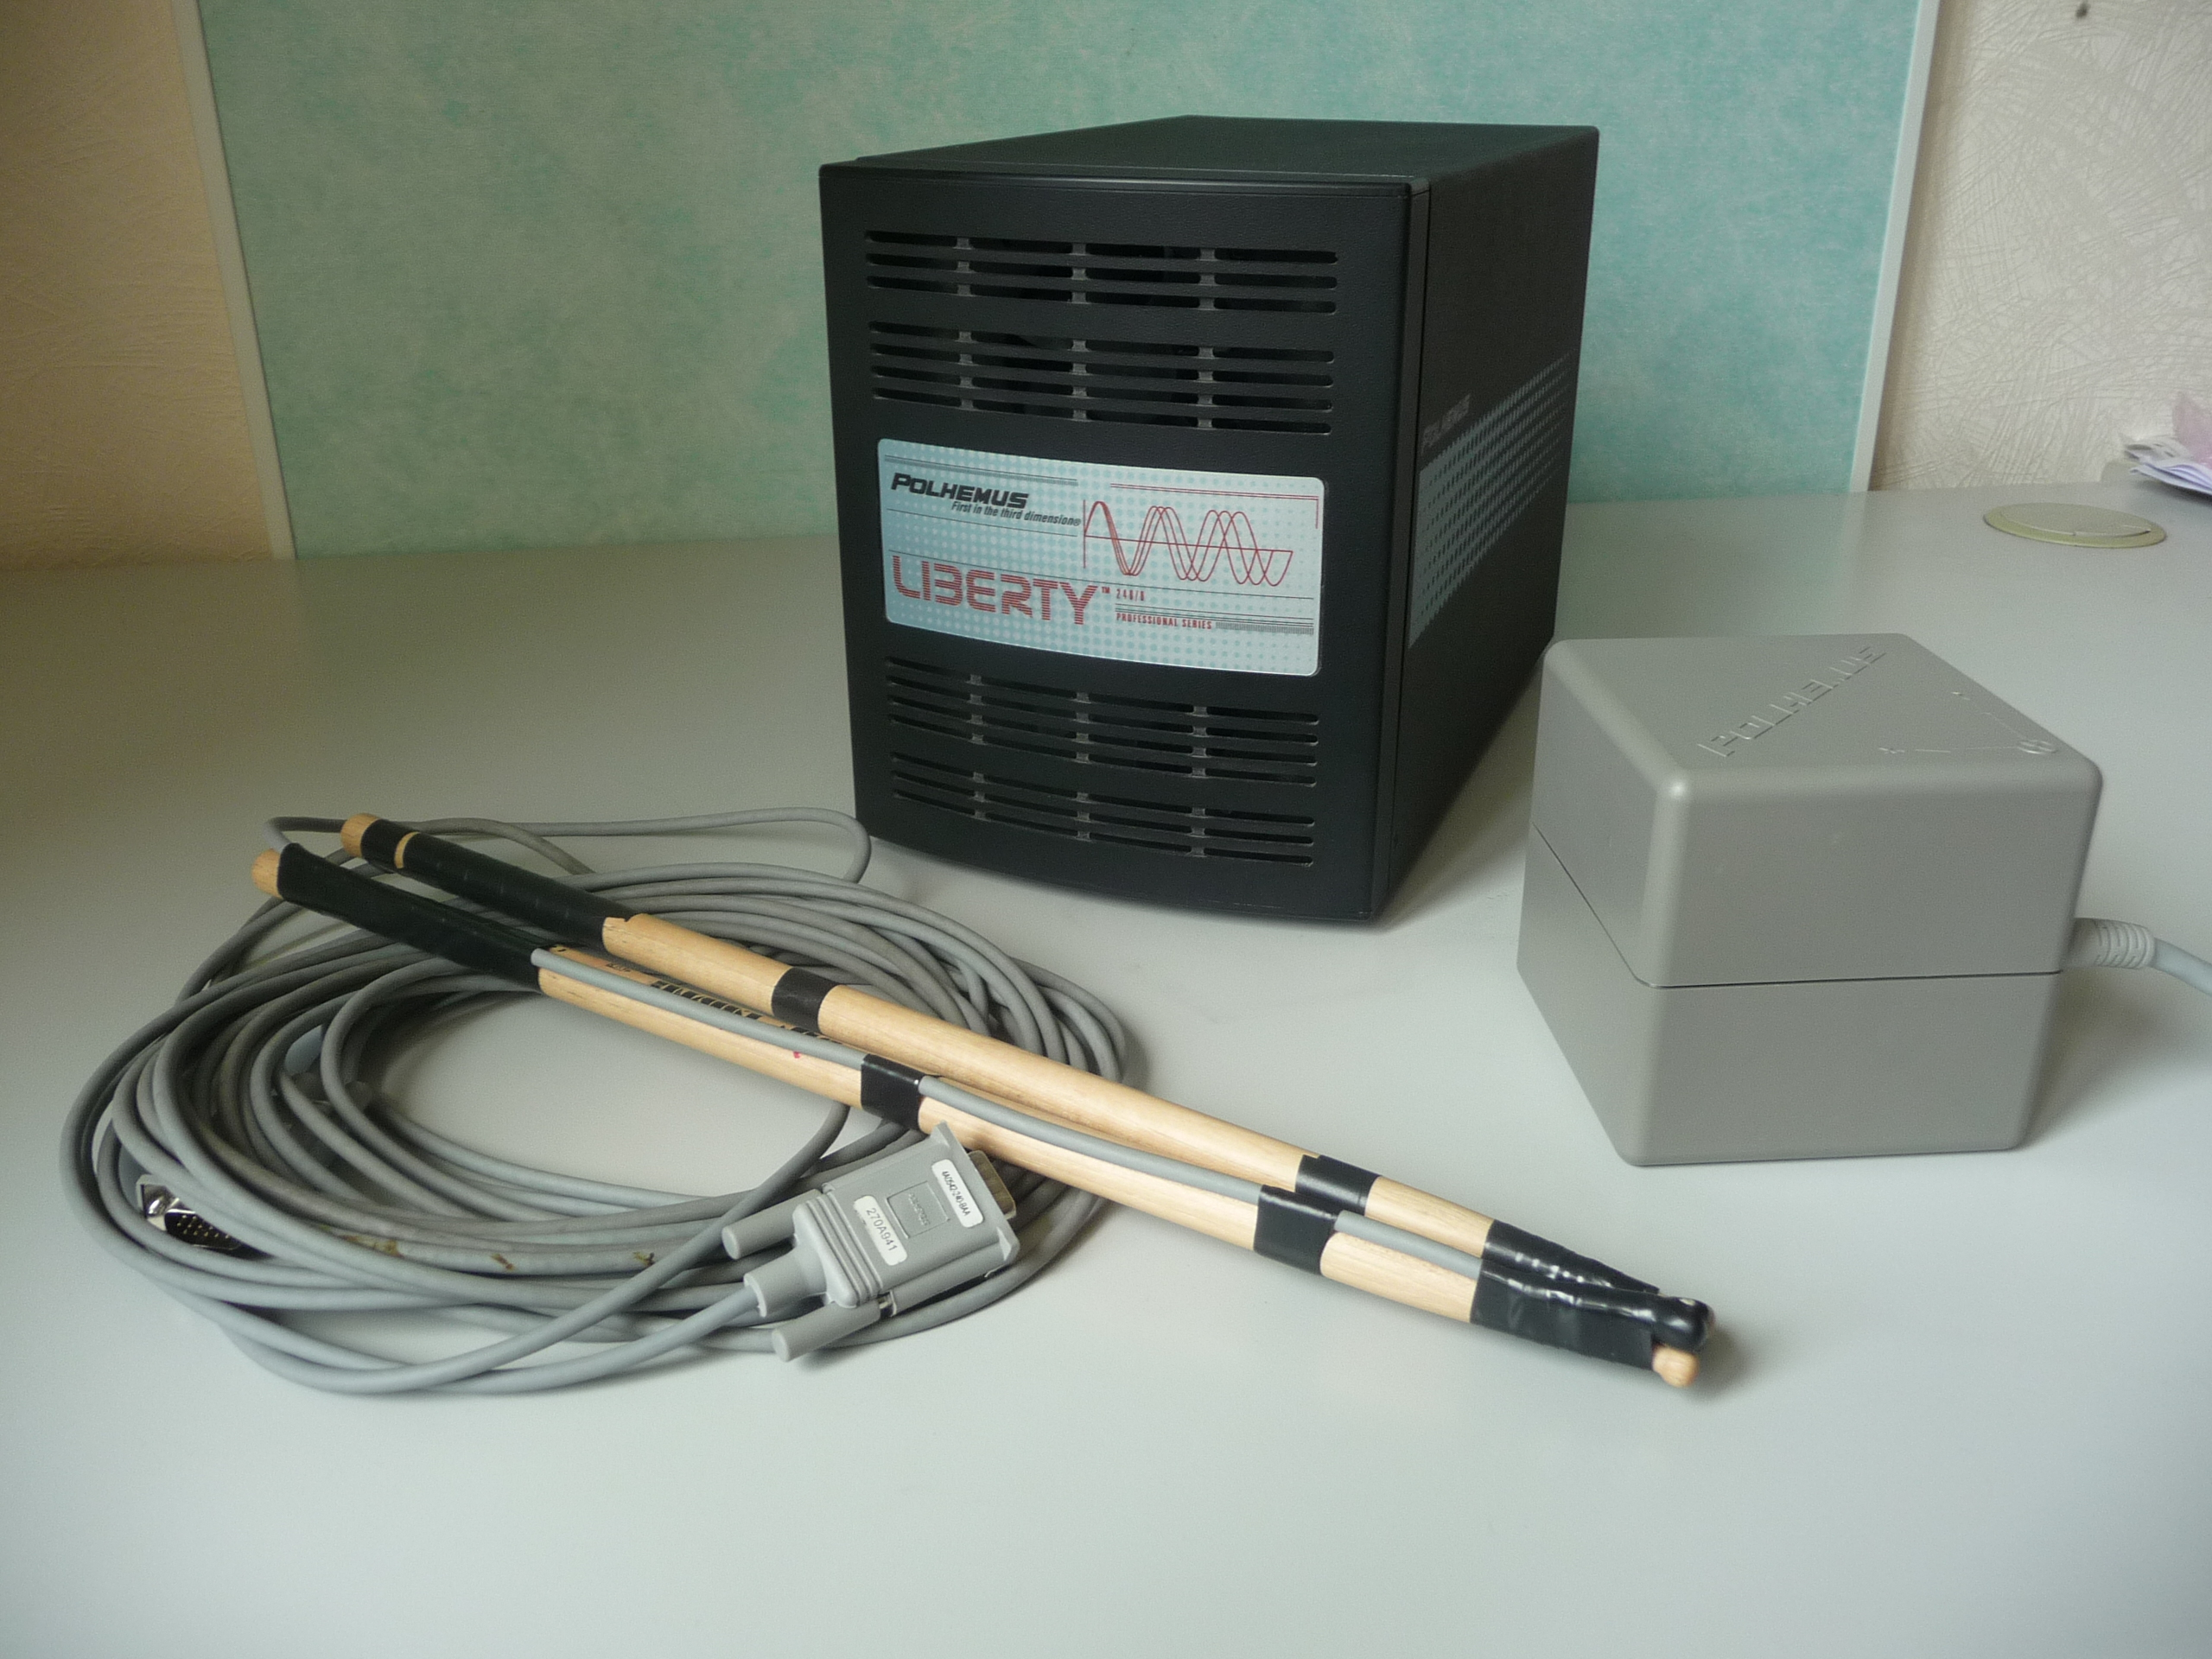
\includegraphics[scale=0.11]{image/percu.jpg}
\caption{Polhemus Liberty and sticks.}
\label{fig:percu}
\end{figure}

\paragraph{}
Mais le dispositif ne fonctionne pas seul. Il y a aussi une couche logiciel.

\subsection{SetKreator and FoB}

SetKreator a été développé au \ac{SCRIME} par Joseph Larralde et Sébastien Lebreton. SetKreator est un éditeur d'instruments virtuels pour la percussion aérienne. Il permet de créer des volumes basiques (parallépipèdes, cylindres...) à l'intérieur d'une sphère représentant la zone d'utilisation des capteurs Polhemus, comme à la figure \ref{fig:setkreator}. Il permet aussi d'associer à chaque forme une synthèse sonore particuliére. Il reçoit les données de position des baguettes par flux OSC (Open Sound Control).

\begin{figure}[h!]
\centering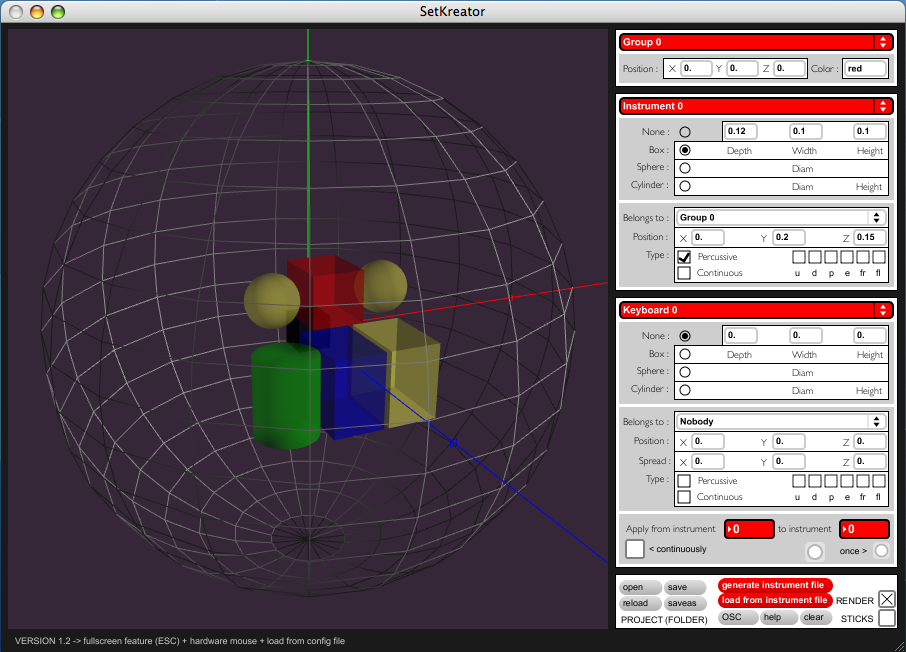
\includegraphics[scale=0.3]{image/setkreator.png}
\caption{Interface of SetKreator}
\label{fig:setkreator}
\end{figure}


Pour faire le lien entre SetKreator et le Polhemus, une autre programme est utile. Il s'agit de FoB. FoB est une petit programme qui reçoit les données de positions du Polhemus via le réseau local de l'ordinateur. Et les renvoie par flux OSC.



\chapter{Realisation}
\section{Objectives}
Apart from the research work, it is asked from us to apply our research to two digital musical instruments (the \brand{Drile} and the Aerial Percussion).

The goal of our work is to enact a live show with these two instruments, that allows for both the performer and the spectators to see the musical instrument in three dimensions.

\subsection{Finding a display}
The first task is to find a suitable display method that would allow : 
\begin{itemize}
\item The performer to interact with the instrument
\item The spectators to see the performer as if he was part of the 3D scene
\item If possible, a stereoscopic feel.
\end{itemize}

\subsection{Implementing suitable renderings}
There is already some existing work for the rendering engine of the Drile, however there is nothing for the aerial percussion.

We have to make renders from two different viewpoints : one for the performer, another for the spectators.

\subsection{Customization}
If we have time left, we are to add some customizations to the aerial percussion rendering, in order to make it look like a real show, with special effects, flares, particles, textures...
\section{Implementation}
We will describe here the multiple choices that have been made during this project, and the reason behind these choices, as well as the result of our implementation.

\subsection{Chosen display techniques}
There are multiple factors to take into account : 
\begin{enumerate}
\item The availability of the technology.
\item The potential price of the required materials.
\item The time to set-up the display.
\item The scaling for a medium-sized audience.
\item The compatibility with the double requirement : a view for the performer, and another for the spectators.
\end{enumerate}

We are now going to study these requirements point by point.
\subsubsection{Availability}
This is the main problem : many of the display devices presented in \ref{chap:3ddisp} have only been the subject of research and not of a real implementation sold by a company (e.g. holograms). Also, the development state of some technologies  might not be sufficient for what we are striving for (e.g. auto stereoscopic displays which are only present in very small screens like smartphones).
\subsubsection{Price}
Some technologies might be irrelevant only because of the amount of money needed to get a working implementation. For instance, an active 84" 3D HDTV generally costs more than ten thousand dollars, which is unsuitable to this project.
\subsubsection{Set-up time}
Some methods might require a very long time to set-up While we don't have a required maximum time to set-up the show, we should try to keep it as low as possible. For instance, the Pepper's Ghost technique is quite long to set-up, because there is a lot of massive hardware, projectors, screens, to set-up.
\subsubsection{Scaling}
Since this is for a show, we need a system that will allow everybody in the room to enjoy the performance. The estimate is at about 40 persons : we need a display that provides big enough viewing angles and is big enough for everybody to be able to enjoy it. A square display with a side of two meters would be ideal to enable complete immersion.
\subsubsection{Double-view requirement}
This is one of the hardest requirements, because it can easily double the quantity of required hardware. For instance, if we were to use 3D TVs, we would need one TV for the viewers and one for the performer.

\subsubsection{The choice}
We chose to go with the Pepper's Ghost technique, with polarized stereo glasses. This was mainly because it was the only method efficiently available with all the tools at our disposal : no additional fees are required.

Due to computer limits, we could not test the two views, but it is implemented in our software. We mainly did focus on the Aerial Percussion, because we did not know how to use the Drile code. 

\subsection{Aerial Percussion implementation}
We will described here the implementation of the Aerial Percussion 3D renderer.

\begin{figure}[h!]
\centering
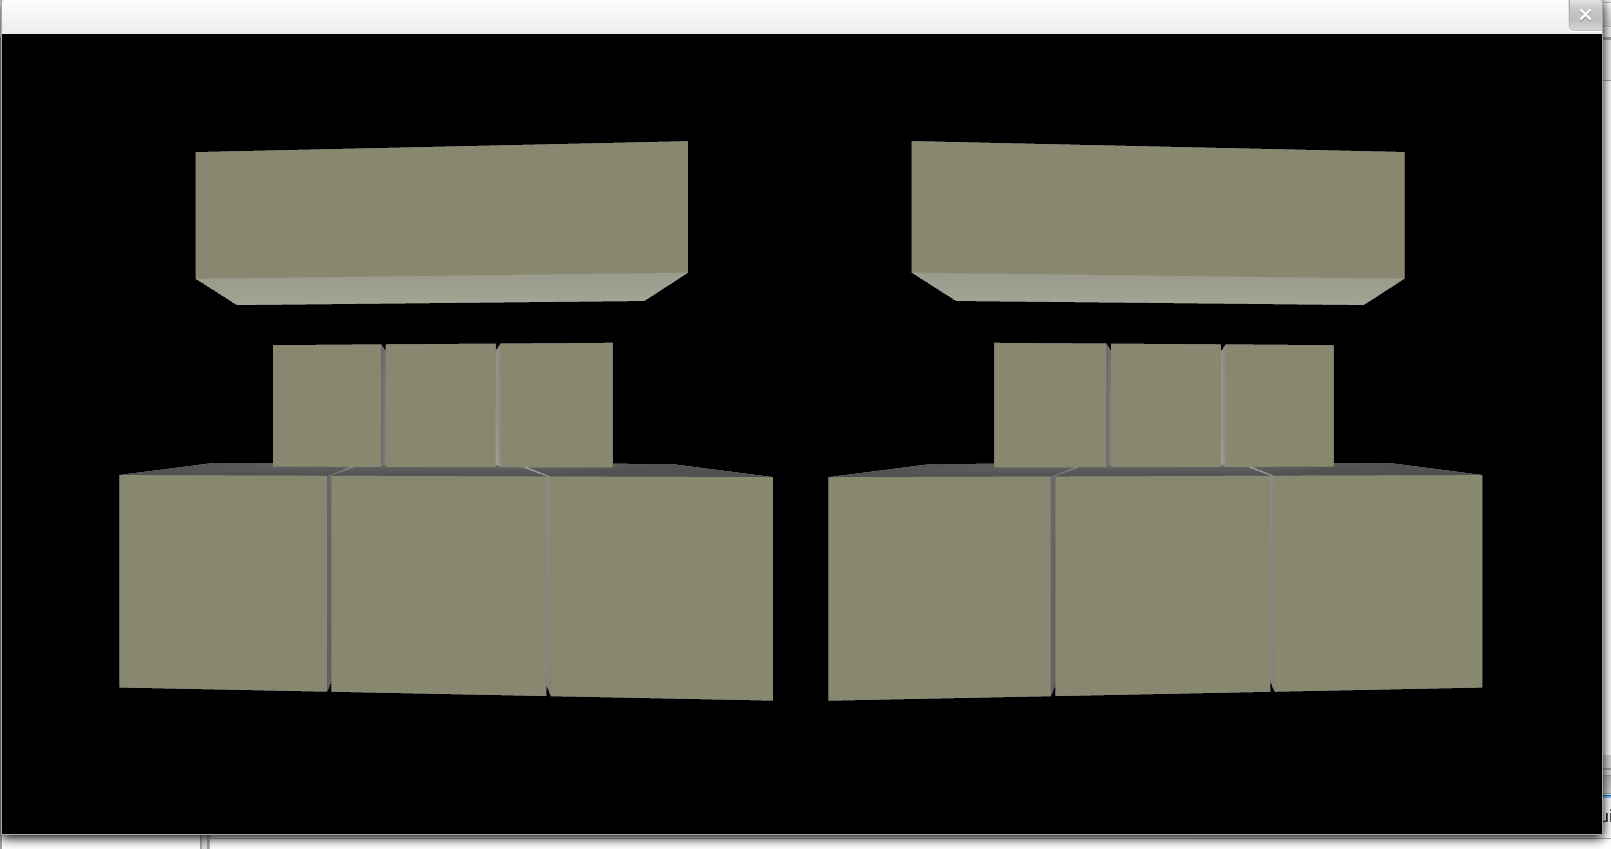
\includegraphics[scale=0.3]{image/percuScreen.png}
\caption{A screenshot of the Aerial Percussion renderer}
\label{fig:percScreen}
\end{figure}

\subsubsection{Technologies used}
We worked with \brand{OpenFrameworks}, a \brand{C++} abstraction over many different media libraries, like \brand{OpenGL}, \brand{OpenNI} and many others. It makes the implementation of creative software easy while retaining the power and speed efficiency of the \brand{C++}.

Our software listens to \brand{OSC} messages, which means that it would be easy to put it on two computers and have one computer display the images for the spectators, and the other for the musician.

\subsubsection{Displaying the data}
\paragraph{Pepper's Ghost technique}
In order to have the Pepper's Ghost technique work efficiently, we have to display our shapes on a black background, so that only the bright parts reflects on the glass screen.

\paragraph{Stereoscopic display}
The method uses two projectors, one on the top of another.
Each projector has a polarizing filter and is connected to a different input of the computer.

The computer, running \brand{Debian GNU/Linux}, is set up so that there is a single viewport of twice a projector's horizontal resolution. Each projector receives one half of the viewport.

For instance, the actual resolution of a projector is $1920 \times 1080$. Hence, the viewport is $3840 \times 1080$.

The software then runs at the same resolution, and the image is displayed from two point of views, that slightly differs on the horizontal axis, as shown on figure \ref{fig:percScreen}. We used frame-buffer objects to achieve this. This allows to generate a 3D effect when the images are projected on the same point in space by the dual projector system, because each eye will receive the correct image, as we could see on paragraph \ref{par:polarized}.

\subsubsection{Additional features}
We added the feature to change the distance between the eyes in order to find the most pleasant one, using the left and right keyboard keys.
We can also zoom in and out using the up and down keys.

The space key will change the point of view from front to back.

The software also reacts by changing the colour of a box when the musician puts a drumstick inside a virtual drum element.

\subsection{Physical set-up of the system}
Figure \ref{fig:schemaPA} presents the set-up for the show.

\begin{figure}[h!]
\centering
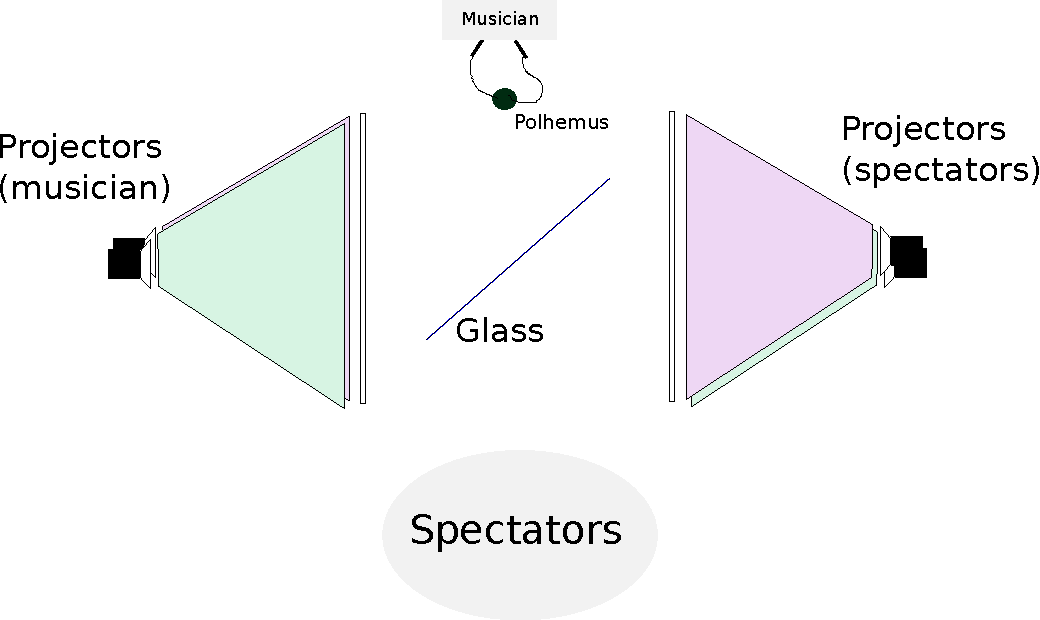
\includegraphics[scale=0.8]{image/schemaPercu.pdf}
\caption{Our installation}
\label{fig:schemaPA}
\end{figure}

\newpage
Figure \ref{fig:percuIRL} shows the result.

The picture is taken from the spectator's point of view. Due to the small size of the glass screen, there are artefacts on the borders. 


\begin{figure}[h!]
\centering
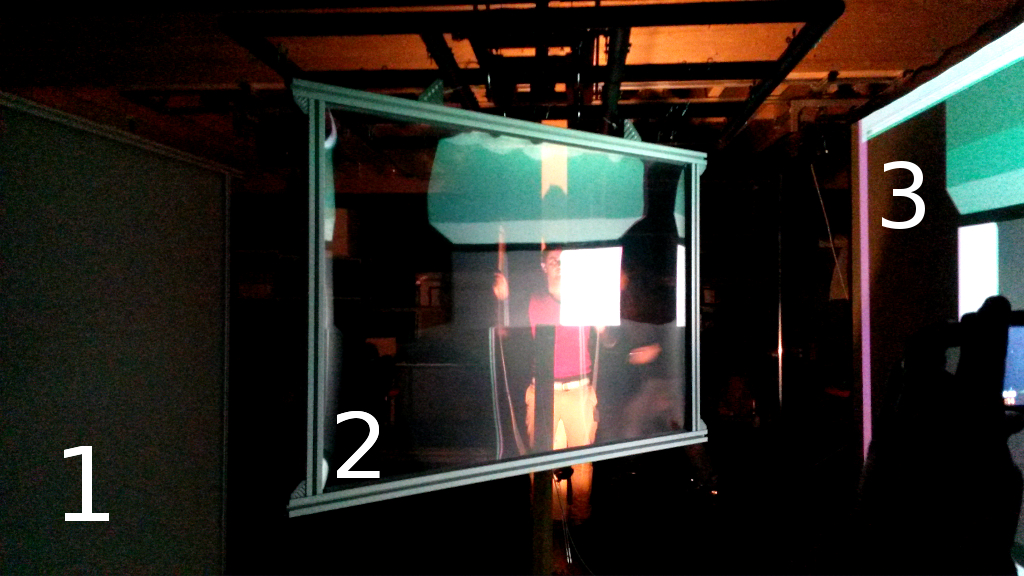
\includegraphics[scale=0.45]{image/percuIRL.jpg}
\caption{Our installation. \textbf{1} and \textbf{3} are the projection screens, \textbf{2} is the Plexiglas screen.}
\label{fig:percuIRL}
\end{figure}

Since the computer only had two video outputs, the system is only able to drive one half of the projectors : here, the spectators half. 

\section{Conclusion}
\begin{frame}
  C'est cool le per
\end{frame}


\printglossaries

\newpage
\begin{itemize}

\item L'article \cite{holliman2011three} 
\item L'article \cite{pimenta2012comprehensive} 
\item L'article \cite{mehrabi2013making} 

\item L'article \cite{kim2012frontal} 

\item L'article \cite{cadoz1999musique} 

\item L'article \cite{berthaut2010piivert}
\item Le livre \cite{okoshi1976three}
\item L'article \cite{rodet2005study} 
\item L'article \cite{plumage2007} 
\item L'article \cite{maki2005} 
\item L'article \cite{wozniewski2006spatial}

\bibliographystyle{alpha}
\bibliography{instru3d}
\end{itemize}
\end{document}
